% Chapter 2

\chapter{Company Presentation} % Main chapter title

\label{Chapter2} % For referencing the chapter elsewhere, use \ref{Chapter2}

\lhead{Chapter 2. \emph{Company Presentation}} % This is for the header on each page - perhaps a shortened title


%----------------------------------------------------------------------------------------

\section{Presentation of Orange}


%----------------------------------------------------------------------------------------

\section{Presentation of Orange Labs}

%----------------------------------------------------------------------------------------
\section{Structure}

%----------------------------------------------------------------------------------------
\section{Team CARE}

%----------------------------------------------------------------------------------------

\subsection{Industrial Radiography Principles}
Industrial radiography is a method for inspecting materials with potentially hidden defects by using the ability of high energy X-rays and gamma rays to penetrate various materials \citep{Reference9}. Industrial radiography is similar to medical X-ray technology in that a film records an image of an item placed between it and a radiation source.


The basic principle of the process is fairly simple and common to all radiography applications (\fref{fig:1}). The radiation from a controlled source penetrates the test item and expose a specially formulated film. As the radiation passes through the item, a portion of it is absorbed by the molecular structure of the material. The amount of radiation absorbed depends on the density and the composition of the material.

\begin{figure}[htbp]
	\centering
		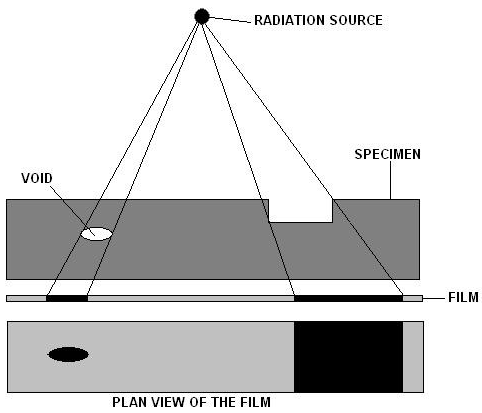
\includegraphics[width=10cm]{Figures/1.png}
	\caption[Industrial Radiography Principle]{Industrial Radiography Principle \citep{irprinciple}.}%{}
	\label{fig:1}
\end{figure}

As cracks, fissures, and any other defects in the material have different densities, they will be characterized by different exposure values as more or less radiation penetrates at those points during exposure. This creates a very accurate image of the internal structure of the item.

At EDF, these techniques are employed to control construction facilities like nuclear power plants, especially metallic components within the primary circuit, the secondary circuit and the cooling system (\fref{fig:2}). The sources of radiation for industrial radiography depend on the process used. At present, EDF utilizes sources of cobalt-60 or iridium-192, which generate gamma radiation. Detectors juxtaposed to the specimen consist of a filter and a cassette with lead shields and one or two silver films (\fref{fig:3}).
\\[1cm]
\begin{figure}[htbp]
	\centering
		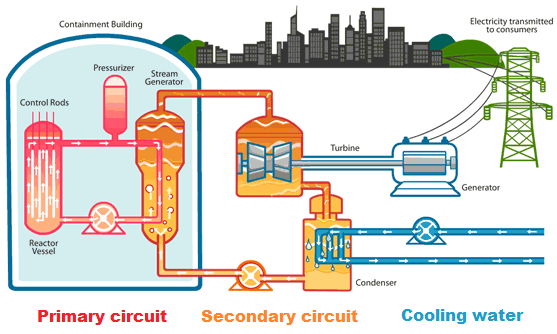
\includegraphics[width=10cm]{Figures/2.png}
	\caption[Mechanism of a nuclear power plant]{Mechanism of a nuclear power plant \citep{plant}.}%
	\label{fig:2}
\end{figure}
\\[1cm]
\begin{figure}[htbp]
	\centering
		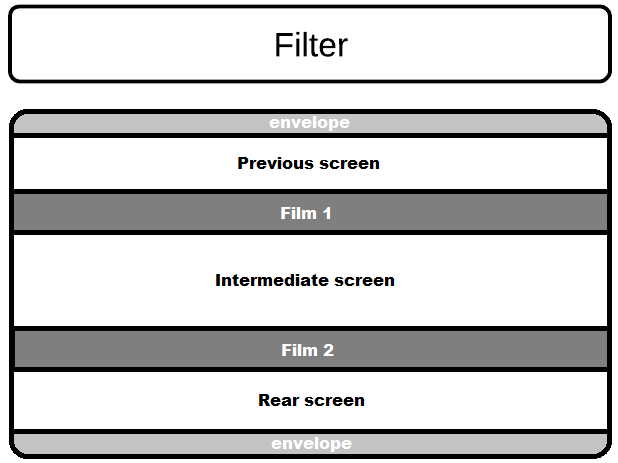
\includegraphics[width=8cm]{Figures/3.png}
	\caption[Detector used by EDF]{Detector used by EDF \citep{Reference10}.}%
	\label{fig:3}
\end{figure}
%----------------------------------------------------------------------------------------

\subsection{Monte-Carlo Modeling Process}
Monte Carlo uses a statistical computing method for solving complex scientific computing problems. It uses random numbers to simulate the uncertainty of inputs to a problem and processes the repeated sampling of the parameter to obtain a deterministic result and solve problems that would otherwise be impossible. This method was originally pioneered by nuclear physicists involved in the Manhattan Project in late 1940s. It is named in reference to the biggest casino in the principality of Monaco.

Compared to deterministic methods that solve the particle transport equation with closed-form expressions, the Monte Carlo method attempts to simulate what happens in reality. When applied to photon transport in MODERATO, it simulates directly single photon's movement by distributing stochastically its energy, direction, free-path and corresponding interactions, from birth to death. This is a straightforward technique that works particularly well when the underlying probabilities of the process are known but the results are more difficult to determine. For example, calculations of risk in finance and business, analysis of quantitative genetics and nuclear reactor simulations, etc.

The essence of the Monte Carlo method is in using a given data-generating mechanism for the process model you wish to understand, produce new samples of simulated data, and examine the results of those samples. Although the modeling process may vary in each individual case, the following procedure would be common to all problems using this method \citep{montecarlo}:
%------------------------------------
\begin{enumerate}
\it
\item Construct a simulated “universe” of randomizing mechanism whose composition is similar to the universe we wish to describe and investigate. The term “universe” refers to the system that is relevant for a single simple event.
\item Specify the procedure that produces a pseudo-sample which simulates the real-life sample in which we are interested. That is, specify the procedural rules by which the sample is drawn from the simulated universe. The simulation procedure must produce simple experimental events with the same probabilities that the simple events have in the real world.
\item If several simple events must be combined into a composite event, describe it in the procedure.
\item Calculate the probability of interest from outcomes of the re-sampling trials.
\end{enumerate}
%------------------------------------
The main drawback in using the Monte Carlo method, however, is that its convergence is governed by the central limit theorem. For many problems, obtaining sufficiently-low statistical error is slow compared to other approaches \citep{Reference2}. This is why any way of accelerating Monte Carlo methods is important for the scientific calculation community and why accelerators like CPU Clusters, MICs, GPGPUs are widely explored in this area. Since the final numerical results are obtained by re-sampling iteratively individual and disjoint events, the Monte Carlo method is well suited to parallel computation in its nature.

%----------------------------------------------------------------------------------------

\subsection{MODERATO Specificities}
MODERATO produces accurate numerical results and predicted images before real examinations, which allows operators to optimize inspection configurations, verify NDT effectiveness and help training technicians \citep{Reference10}. Areas with heat and radioactivity (inside a reactor for example) can be inaccessible to operators. Therefore, MODERATO will be employed to analyze the test and help determining an optimal configuration. Without a simulation tool like this, the operation can be both dangerous and costly. Another function of MODERATO is to qualify test methods. The code simulates operating process and checks if the method can meet expected needs: can this method find potential defects? Is it capable of locating them all? Since real radiographic tests cost a lot, a qualification before using is very profitable. So as to train inspection controllers, MODERATO plays an important role as well. Although this virtual simulation never replaces real practice, it makes technicians quickly get a preview of their work and have better awareness on the whole operation.

The simulations of a radiographic inspection used by EDF pose particular problems, and none of the existing codes at that time can solve them well. As a result, in order to satisfy all these specificities, MODERATO was created with following features \citep{Reference10}:
%------------------------------------
\begin{itemize}
  \it
  \item \textbf{Handle the thickness of inspected objects and manage to simulate interactions inside.}
  \item \textbf{Model the specific detector with several films and metal screens.} Note that characteristics of each film vary a lot, a microscopic modeling is necessary instead of a macroscopic one with experimental calibration of a large number of transfer functions. However, this work had never been done before MODERATO. Moreover, the modeling of the rear screen within detectors is rather delicate \citep{Reference10}.
  \item \textbf{Deal with complex geometries.} Analytical parameterized geometries are described precisely by their borders. Using the \textit{CADSurface} and \textit{CADContour} system, MODERATO is capable of compositing many complex geometries with several basic ones.
\end{itemize}
%------------------------------------

%----------------------------------------------------------------------------------------

\section{Parallelization with Various Architectures}
The development of MODERATO has begun since the end of 1990s when parallel computing was not commonly used like nowadays. The original implementation was a scalar one which processed a single pair of operands at a time. Then, parallelism work has been done during the past years, which converts the single-process source code to a multi-process one.

Parallelization of MODERATO was realized with MPI (Message Passing Interface): a major computing process is responsible for centralizing all other processes by distributing them with data and then collecting it back. The whole process from generating photons to simulating their multi-diffusions within inspected objects is treated by sub-processes. Afterwards, all photons which succeed in reaching the detector are sent back to the major process which performs the detector treatments: modeling films, generating result files, etc. In theory, the gain of this parallelization is proportional to the number of sub-units: a certain number of sub-units may bring almost the same amount of speedup.

Although hardware accelerators is a relatively rising technology, there has been much research about porting radiographic Monte Carlo on it. Among all these work, a group at Rensselaer Polytechnic Institute in USA has made significant achievement \citep{xu2013update, liu2014comparison, su2014archerrt, liu2013tu}. They developed a fast Monte Carlo code ARCHER (Accelerated Radiation-transport Computation in Heterogeneous EnviRonments) to model medical CT (Computed Tomography) imaging process on heterogeneous computing systems (or hardware accelerators). Simulating the transport of low-energy (1$\sim$140keV) photons, ARCHER contains three code variants: ARCHER-CTcpu, ARCHER-CTgpu and ARCHER-CTcop to run in parallel on the multi-core CPU, GPU and coprocessor architectures respectively. These three versions have been developed correspondingly in MPI-OpenMP, CUDA and offload OpenMP. According to their study, the ARCHER results agreed well with those from the production code Monte Carlo N-Particle eXtended (MCNPX). It was found that all the code variants were significantly faster than the parallel MCNPX running on 12 MPI processes, and that the GPU and coprocessor performed equally well, being 2.89$\sim$4.49 and 3.01$\sim$3.23 times faster than the parallel ARCHER-CTcpu running with 12 hyper-threads cores \citep{liu2014comparison}. The three computing architectures mentioned above will be presented in the following of this section.

%----------------------------------------------------------------------------------------

\subsection{CPU Clusters}
A computer cluster is a single logical unit consisting of multiple computers that are linked through a LAN (Local Area Network). The networked computers essentially act as a single, much more powerful machine. The major advantages of using computer clusters are \citep{cluster}:
\begin{itemize}
\it
\setstretch{1} % Reset the line-spacing to 1
\item \textbf{Cost efficiency: }the cluster technique is cost effective for the amount of power and processing speed being produced. It is more efficient and much cheaper compared to other solutions like setting up mainframe computers.
\item \textbf{Processing speed: }multiple high speed computers work together to provided unified processing, and thus faster processing overall.
\item \textbf{Improved network infrastructure: }different LAN topologies are implemented to form a computer cluster. These networks create a highly efficient and effective infrastructure that prevents bottlenecks.
\item \textbf{Flexibility: }unlike mainframe computers, computer clusters can be upgraded to enhance the existing specifications or add extra components to the system.
\item \textbf{High availability of resources: }If any single component fails in a computer cluster, the other machines continue to provide uninterrupted processing. This redundancy is lacking in mainframe systems.
\end{itemize}
So as to benefit the advantages, parallel MODERATO was recently tested by {\supname} on a new EDF R\&D cluster (ATHOS) with few changes of original source code. Test results show that MODERATO is greatly accelerated with large-scale parallelism, further details about this test will be presented in \sref{optixperform}.
%----------------------------------------------------------------------------------------
\subsection{Intel MIC}
Intel Many Integrated Core Architecture (or Xeon Phi) is a coprocessor computer architecture running its own operating system. The coprocessor core implements most of the new instructions associated with 64-bit extension. However, the only vector instructions supported are the initial Intel Many Core Instruction set. There is no support for Intel MMX technology, Intel SSE, or Intel AVX in the coprocessor cores, although the scalar math unit (x87) remains integrated and fully functional.

MIC provides an ideal execution vehicle for Monte Carlo-related applications. Building around the x86-64 instruction set architecture, using the very same programming model as the other multi-core processors, Xeon Phi extends the parallel execution infrastructure with little or no modification of source code, according to an Intel developer \citep{micdeveloper}. The main advantage of using MIC, with respect to other co-processors and accelerators, is the simplicity of the porting \citep{Bernaschi20142495}. Programmers do not have to learn a new programming language but may compile their source codes specifying MIC as the target architecture. The classic programming languages (HPC-Fortran, C, C++) as well as the parallel paradigms: OpenMP or MPI-may be directly employed regarding MIC as a “classic” x86 based (many-core) architecture.

Aside from ARCHER, there are few studies on performing Monte Carlo particle transport on Xeon Phi. The only research team I found in this area focuses on proton transport in Monte Carlo codes \citep{souris2014th, sterpin2014180}. It is worth noting that because of its totally new vector processing unit, porting work on MIC with numerous vector operations may not be more straightforward than that on GPGPU.
%----------------------------------------------------------------------------------------

\subsection{GPGPU}
General-purpose computing on graphics processing units is to use the initial rendering graphics GPU for normal computation. Compared to CPUs, they have a higher aggregate memory bandwidth, much higher FLoating-point Operations Per Second (FLOPS), and lower energy consumption per FLOP \citep{Reference2}. Because one of the main obstacles in exascale computing is power consumption, many new supercomputing platforms are gaining much of their computational capacity by incorporating GPUs into their compute nodes.

A study led by Martinsen concerns with modeling photon transport in anisotropy media on using CUDA architecture \citep{Reference1}. Their implementation, processing roughly 110 million scattering events per second, was found to run more than 70 times faster than a similar, single-threaded implementation on a 2.67 GHz desktop computer.

Tickner \citep{Reference3} has implemented a general-purpose code that computes the transport of high energy photons through arbitrary 3-D geometry models, simulates their physical interactions and performs tallying and variance reduction. It describes a new algorithm that provides a good match with the underlying GPU multiprocessor hardware design. Benchmarking against an existing CPU-based simulation running on a single-core of a commodity desktop CPU demonstrates that the code can accurately model X-ray transport, with an approximately speed-up factor of 35.

Furthermore, Kalantzis and Tachibana \citep{tachibana2014accelerated} carried out a study of hybrid (OpenMP and CUDA) MC tracking implementation. A maximum speedup of 67.2 (compared to a single threaded CPU version) was achieved for the primary GPU-based MC code, while a further improvement of the speedup up to 20\% was achieved for the hybrid approach. The results indicate the encouraging capability of this CPU–GPU implementation for accelerated MC calculations of particle tracks without loss of accuracy.

According to these significant results, we conclude that GPGPU is a powerful accelerator for scientific computing. These speedup factors make it very attractive to use in extremely parallel, computationally-intensive Monte Carlo simulations.

%----------------------------------------------------------------------------------------

\section{Specific Ray Tracing Engines}
An essential part of MODERATO is its ray tracing package, which is in charge of tracking the entire trajectory of every photon and accelerating with bounding boxes. Given that the photon histories are completely independent, this tracking model fits perfectly parallel accelerators. However, even if parallelization is easy, efficient vectorization is hard since it requires deep knowledge about hardware architecture. The typical ray tracing algorithms can be highly irregular, which poses serious challenges for anyone trying to exploit the full raw computational potential of a computing accelerator \citep{Reference6}. Consequently, several specific ray tracing engines address those challenges and provide frameworks for harnessing the enormous computational power of the accelerator to incorporate ray tracing into interactive applications. In this manner, interactive ray tracing is finally feasible for developers without a Ph.D. in HPC and a team of ray tracing engineers.

%----------------------------------------------------------------------------------------

\subsection{Intel Embree}
Embree is an open source ray tracing framework for x86 CPUs \citep{wald2014embree}. Although it's an API explicitly designed to achieve high performance in professional rendering environments, it's said that Embree doesn't limit within a complete rendering application. In addition, the manual \citep{embree} emphasizes that its ray tracing kernel has been optimized for incoherent Monte Carlo ray tracing algorithms.

Embree is a cross-platform API: Windows, Linux and Mac OS X are all supported in both 32bit and 64bit modes. In particular, the Xeon Phi version is only available in 64-bit Linux distribution.

In terms of geometry description, both triangle meshes and analytical methods are supported. Users may choose either a dynamic or a static way to establish geometry primitives. Like OptiX, Embree also provides automatic acceleration structures for the ray tracing process, but this acceleration is relatively simple. Users select a tracing mode (coherent, incoherent, robust, etc.) instead of specifying a particular structure in OptiX. Moreover, bounding box of meshes are automatically built by Embree ray tracing mechanism. Embree supports \textit{Hair Geometry} as a geometry mode, which consist of multiple curves represented as the cubic Bézier curve with varying radius per control point. This new feature may be helpful to describe more accurate \textit{CADContour} in MODERATO.

Ray tracing mechanism in Embree is similar to OptiX, it supports finding the closest hit point of a ray segment with \textit{rtcIntersect} functions, and determining if any intersection point exists by using \textit{rtcOccluded}. The API supports per geometry Embree \textit{Filter} callback functions that are invoked for each intersection found during the \textit{rtcIntersect} or \textit{rtcOccluded} calls. However, the \textit{Filter} function is only supported for triangle mesh geometry. Since ray reflections or refractions in rendering graphic necessitate such functions to change ray directions and cast new rays, we would like to investigate it for analytical geometries before modeling the photon interaction.

Even if the manual says that the API provides a low-level ray tracing mechanism, further investigation is required to make clear how to combine the ray tracing kernel with general programs. Note that Embree has been proposed since two years ago and as far as I know, until now, there is no paper published concerning Embree for Monte Carlo simulations. This may imply it's not suitable for general-purpose calculations.
%----------------------------------------------------------------------------------------

\subsection{NVIDIA OptiX}
As a more specific GPGPU extension, OptiX provides a basic and scalable ray tracing framework for graphics as well as general-purpose computing. Wherever possible, OptiX avoids specification of ray tracing behaviors and instead provides mechanisms to execute user-provided CUDA C code \citep{Reference6}. This low-level support focuses exclusively on the fundamental computations required for ray tracing and avoids embedding rendering-specific constructs. The engine presents mechanisms for expressing ray-geometry interactions and does not have built-in concepts of lights, shadows, reflectance, etc \citep{Parker10OptiX}.

Geometry representation within OptiX is extremely flexible and agrees well to the request of MODERATO: both analytical methods and mesh methods are available. It's users themselves that describe geometries as well as corresponding intersections and interactions. OptiX just provides a ray tracing interface between user-supplied programs and GPGPU architectures. Besides this flexibility, OptiX provides optimizations that may take months for developers to replicate by themselves. Its main advantage is automatically creating high-quality acceleration structures for traversing the primitives in a geometry scene \citep{Reference6}.

OptiX Prime was integrated in OptiX since the 3.5 version. Being compared with OptiX, the Prime is a more low-level API for applications which are just designed to find intersections. On removing all features around rendering and shading, OptiX Prime handles meshes and rays and it returns the intersections at over 300 million rays per second on a single GPU \citep{optixgroup}. What interests us more is that OptiX Prime also provides an efficient CPU fallback when a suitable GPU is not present. However, analytical parameterized geometries are no more supported, which would be a main drawback for using it to optimize MODERATO. Another concern is that commercial applications require a commercial license to redistribute OptiX 3.5 and later editions. Since the use of MODERATO is not restricted within EDF, additional cost for licenses will pressure its commercial use.

One can find some researches on using OptiX for scientific Monte Carlo simulations. Bergmann, now post-doc at Nuclear Engineering Department of UC Berkley, just finished his dissertation on developing a framework for continuous energy Monte Carlo neutron transport on GPUs. The framework, which is called WARP, accelerates Monte Carlo simulations while preserving the benefits of Monte Carlo method. Optimized, high-performance GPU libraries such as CUDPP (CUDA Performance Primitives: performing parallel reductions, sorts and sums), CURAND and OptiX are used wherever possible \citep{Reference2}. In an initial testing where 106 source neutrons per criticality batch are used, WARP produces results agreeing well with that of MCNP 6.1 and Serpent 2.1.18 and takes much less computation time. He concludes that WARP’s performance on a NVIDIA K20 is equivalent to approximately 45 AMD Opteron 6172 CPU cores.

Other researches draw conclusions similar to that of Bergmann \citep{gpuconf, Safari2014101}: OptiX presents remarkable tracking performance as well as promising agreements with reference MC codes, for example, MCNP and GEANT4. They emphasized that by using OptiX, GPU implementation problems like keeping all available GPUs busy, minimizing memory transfers and optimizing use of hardware will be automatically solved.

%----------------------------------------------------------------------------------------
